\title{Study Guide for Midterm 1}
\author{Dr. Jordan Hanson - Whittier College Dept. of Physics and Astronomy}
\date{\today}
\documentclass[10pt]{article}
\usepackage[a4paper, total={18cm, 27cm}]{geometry}
\usepackage{outlines}
\usepackage{graphicx}
\begin{document}
\maketitle

\textbf{Instructions:} Work each problem \textit{before} checking your answer with the key (to follow on Moodle). \\ \vspace{0.25cm}

\section{Memory Bank}

\begin{enumerate}
\item $m = \rho V$ ... Mass is the density times the volume
\item $V = \frac{4}{3}\pi r^3$ ... The volume of a sphere
\item $\vec{F} = k \frac{q_1 q_2}{r^2}\hat{r}$ ... Coulomb Force
\item $k = 9 \times 10^{9}$ N C$^{-2}$ m$^{2}$ ... Remember $k = 1/(4\pi \epsilon_0)$.
\item $q_e = 1.6 \times 10^{-19}$ C ... Charge of an electron/proton
\item Atomic mass: the number of grams per mole of a substance
\item $N_A = 6.03 \times 10^{23}$ ... Avagadro's number
\item $\vec{F} = q \vec{E}$ ... Electric field and charge
\item $\vec{E}(z) = \frac{\sigma}{\epsilon_0}\hat{z}$ ... Electric field of two oppositely charge planes each with charge density $\sigma$
\item $\epsilon_0 \approx 8.85 \times 10^{-12}$ F/m
\item $dE = \int k dq / r^2$ ... Remember that $dq$ takes the form below
\item $dq = \lambda dx$ ... Linear charge density (C/m)
\item $\vec{E}(z) = \frac{1}{4\pi\epsilon_0} \frac{2\lambda}{z} \hat{k}$ ... Electric field above an infinite line of charge with charge density $\lambda$
\item $\vec{E} \cdot \vec{A} = Q_{enc}/\epsilon_0$ ... Gauss' Law, constant electric field over the surface area.
\item $U = q\Delta V$ ... Potential energy and voltage
\item 1 eV: an electron-Volt is the amount of energy one electron gains through 1 V.
\item $V(r) = k\frac{q}{r}$ ... Voltage of a point charge
\item $\vec{E} = -\frac{\Delta V}{\Delta x}$ ... E-field is the slope or change in voltage with respect to distance.
\item $\vec{E} = -\nabla V$ ... General relationship between E-field and potential.
\item $\nabla V(x,y,z) = \frac{\partial V}{\partial x}\hat{i} + \frac{\partial V}{\partial y}\hat{j} + \frac{\partial V}{\partial z}\hat{k}$
\item $V(x) = -E x + V_0$ ... Voltage is linear between two charge planes
\item $Q = CV$ ... Definition of capacitance
\item $C = \frac{\epsilon_0 A}{d}$ ... Capacitance of a parallel plate capacitor
\item $C_{tot}^{-1} = C_1^{-1} + C_2^{-2}$ ... Adding two capacitors \textit{in series.}
\item $C_{tot} = C_1 + C_2$ ... Adding two capacitors \textit{in parallel.}
\item $U = \frac{1}{2}CV^2$ ... Stored energy in capacitors.
\item $w = mg$ ... Weight force, given gravitational acceleration.
\item $\vec{F}_{\rm net} = m\vec{a}$ ... Newton's second law.
\end{enumerate}

\clearpage

\section{Electric Charge and Electric Fields}

\begin{enumerate}
\item \textbf{Scaling problem}: (a) Some point charge produces an E-field $E_{\rm C} = 2.00 \times 10^{-3}$ V/m at a distance of 1 mm. What is the value of $E_{\rm C}$ at 5 mm produced by the same charge? (b) A 1 $\mu$C charge produces an E-field $E_{\rm C} = 8.00 \times 10^{-3}$ V/m at some distance.  What is the value of $E_{\rm C}$ at the same distance if the charge is 3 $\mu$C? \\ \vspace{1cm}
\item 
\begin{figure}
\centering
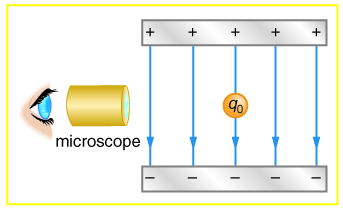
\includegraphics[width=0.3\textwidth]{mill.jpeg}
\caption{\label{fig:mill} The classic Millikan oil drop experiment was a measurement of the charge of an electron.}
\end{figure}
The classic Millikan oil drop experiment was the first to measure the electron charge. Oil drops were suspended against the gravitational force by an electric field. (See Fig. \ref{fig:mill}.) Suppose the drops have a \textit{mass} of $4\times 10^{-16}$ kg, and the E-field is oriented downward, and has a value of 6131.25 N/C.  With this exact value, the drops remain suspended in air.  (a)  How many electrons are on the drops?  (b) Suppose a cosmic ray comes along and removes an electron from a droplet.  What will the acceleration of the droplet be? \\ \vspace{3cm}
\item Consider the charges in Fig. \ref{fig:tri}.  We know some molecules have a charge distribution similar to Fig. \ref{fig:tri}, because they can be polarized.  (a) What is the electric field \textbf{vector} at point M, in terms of $q$ and $a$?  \textit{Check your units.} (b) If the q's are electrons, and $a = 10^{-10}$ m, what is the value of the E-field at point M?  (c) \textbf{Bonus point:} Imagine a point P that is a distance $r \gg a$ from the triangle.  What should the E-field be, in terms of $q$ and $a$?
\begin{figure}[ht]
\centering
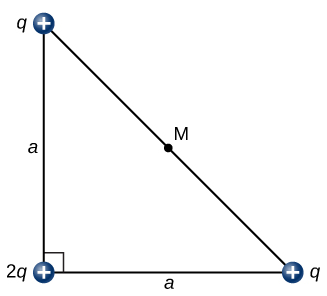
\includegraphics[width=0.25\textwidth]{charges1.png}
\caption{\label{fig:tri} A right triangle, $a = 0.1$ nm.}
\end{figure} \\ \vspace{1cm}
\item A very long, thin wire has a uniform linear charge density of 50 $\mu$C/m.  What is the electric field at a distance 2.0 cm from the wire?  \textbf{Bonus point}: Prove using Gauss' Law.  \\ \vspace{2cm}
\end{enumerate}

\section{Potential Energy and Voltage}

\begin{enumerate}
\item A \textit{mass spectrometer} is a device used to accelerate ions to determine atomic masses of chemicals.  Suppose two conducting plates with potential difference $\Delta V = 4$ kV are used to accelerate both hydrogen ions and helium ions.  Hydrogens have charge $+1 q_e$, and helium ions have charge $+2 q_e$.  (a) What is the total kinetic energy (in electron-volts) gained by the hydrogens and heliums? (b) If the plate separation is $\Delta x = 5$ cm, what is the electric field value?  \textit{Hint: think of the E-field as the slope of voltage.} \\ \vspace{3cm}
\item Suppose a parallel plate capacitor is formed from a positive plate and a negative plate of charge.  Potential difference between the plates is 5 V.  (a) If the separation between the plates is 5 mm, what is the electric field between the plates? (b) If we \textit{decide} that 0V corresponds to the negative plate, at what distance from the positive plate is the potential 4 V?  \textit{Graph $V(x)$ if you're note sure.} (c) Suppose the positive plate is above the lower plate, and that an electron sails through the volume between the plates, and exits.  Is the path of the electron directed upwards or downwards? \\ \vspace{3.5cm}
\end{enumerate}

\section{Capacitors}

\begin{enumerate}
\item (a) What is the total capacitance in Fig. \ref{fig:caps1}?  \textit{Think of them as one big capacitor}. (b) If the potential difference across them is 5V, what is the total stored charge? (c) What is the total stored energy? 
\begin{figure}[hb]
\centering
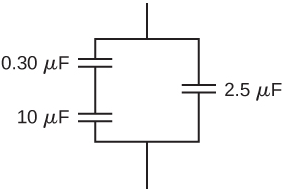
\includegraphics[width=0.3\textwidth]{caps1.png}
\caption{\label{fig:caps1} A network of capacitors connected together.}
\end{figure}
\end{enumerate}

\end{document}